\documentclass[12pt]{article}
\usepackage{amsmath, amssymb}
\usepackage{geometry}
\usepackage{enumitem}
\usepackage{tikz}
\geometry{margin=1in}

\title{Washer and Shell Method Practice}
\author{}
\date{}

\begin{document}
\maketitle

\section*{Instructions}
Complete within 60 minutes. Show setup clearly before integrating. Use exact values unless a decimal approximation is explicitly requested.

\section*{Relevant Formulas}
\[
V_{\text{washer}}=\pi\int_a^b \Big(R(x)^2-r(x)^2\Big)\,dx
\qquad
V_{\text{shell}}=2\pi\int_a^b (\text{radius})(\text{height})\,dx
\]
\[
V_{\text{washer}}=\pi\int_c^d \Big(R(y)^2-r(y)^2\Big)\,dy
\qquad
V_{\text{shell}}=2\pi\int_c^d (\text{radius})(\text{height})\,dy
\]

\begin{center}
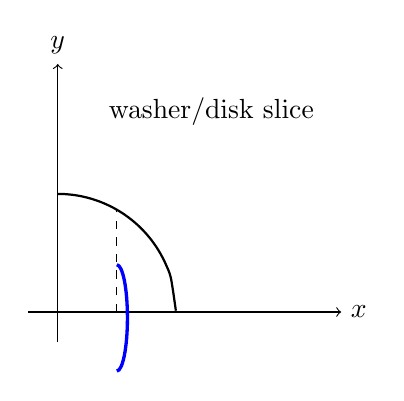
\begin{tikzpicture}[scale=0.75]
  \draw[->] (-0.5,0) -- (4.8,0) node[right] {$x$};
  \draw[->] (0,-0.5) -- (0,4.2) node[above] {$y$};
  \draw[thick,domain=0:2,smooth] plot(\x,{sqrt(4-\x*\x)});
  \draw[thick] (0,0)--(2,0);
  \draw[dashed] (1,0) -- (1,{sqrt(3)});
  \draw[very thick,blue] (1,0.8) arc[start angle=90,end angle=-90,x radius=0.18,y radius=0.9];
  \node at (2.6,3.4) {washer/disk slice};
\end{tikzpicture}
\hspace{0.8cm}
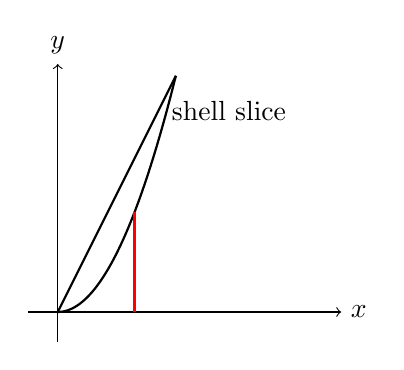
\begin{tikzpicture}[scale=0.75]
  \draw[->] (-0.5,0) -- (4.8,0) node[right] {$x$};
  \draw[->] (0,-0.5) -- (0,4.2) node[above] {$y$};
  \draw[thick,domain=0:2,smooth] plot(\x,{\x*\x});
  \draw[thick] (0,0)--(2,4);
  \draw[dashed] (1.3,0) -- (1.3,{1.69});
  \draw[very thick,red] (1.3,0) -- (1.3,1.69);
  \node at (2.9,3.4) {shell slice};
\end{tikzpicture}
\end{center}

\section*{Problems}
\begin{enumerate}[leftmargin=*, itemsep=1em, topsep=0.8em]
  \item Find the volume obtained by rotating the region bounded by $y=x^2$, $y=0$, and $x=2$ about the $x$-axis.

  \item Find the volume obtained by rotating the region bounded by $y=\sqrt{x}$, $y=0$, and $x=4$ about the $x$-axis.

  \item Find the volume obtained by rotating the region bounded by $y=x$ and $y=x^2$ about the $x$-axis.

  \item Find the volume obtained by rotating the region bounded by $y=2x-x^2$ and $y=0$ about the $y$-axis using the shell method.

  \item Find the volume obtained by rotating the region bounded by $y=x^3$, $x=0$, $x=1$, and $y=0$ about the $y$-axis using the shell method.

  \item Find the volume obtained by rotating the region bounded by $y=4-x^2$ and $y=0$ about the $y$-axis using the washer method.

  \item The region bounded by $y=x^2$ and $y=2x$ is revolved about the line $y=-1$. Find the volume.

  \item The region bounded by $y=\sqrt{x}$, $y=0$, and $x=9$ is revolved about the line $y=3$. Find the volume.

  \item The region bounded by $x=y^2$ and $x=2y$ is revolved about the $y$-axis. Find the volume using washers.

  \item The region bounded by $x=y^2$ and $x=6-y$ is revolved about the $y$-axis. Find the volume using washers.

  \item The region bounded by $y=x$ and $y=x^2$ is revolved about the line $x=2$. Find the volume using shells.

  \item The region bounded by $y=\ln x$, $y=0$, and $x=e$ is revolved about the $y$-axis. Find the volume using shells.
\end{enumerate}

\end{document}
